% Options for packages loaded elsewhere
\PassOptionsToPackage{unicode}{hyperref}
\PassOptionsToPackage{hyphens}{url}
%
\documentclass[
  12pt,
  a4paper,
  DIV=11,
  numbers=noendperiod]{scrreprt}

\usepackage{amsmath,amssymb}
\usepackage{setspace}
\usepackage{iftex}
\ifPDFTeX
  \usepackage[T1]{fontenc}
  \usepackage[utf8]{inputenc}
  \usepackage{textcomp} % provide euro and other symbols
\else % if luatex or xetex
  \usepackage{unicode-math}
  \defaultfontfeatures{Scale=MatchLowercase}
  \defaultfontfeatures[\rmfamily]{Ligatures=TeX,Scale=1}
\fi
\usepackage{lmodern}
\ifPDFTeX\else  
    % xetex/luatex font selection
\fi
% Use upquote if available, for straight quotes in verbatim environments
\IfFileExists{upquote.sty}{\usepackage{upquote}}{}
\IfFileExists{microtype.sty}{% use microtype if available
  \usepackage[]{microtype}
  \UseMicrotypeSet[protrusion]{basicmath} % disable protrusion for tt fonts
}{}
\usepackage{xcolor}
\setlength{\emergencystretch}{3em} % prevent overfull lines
\setcounter{secnumdepth}{5}
% Make \paragraph and \subparagraph free-standing
\makeatletter
\ifx\paragraph\undefined\else
  \let\oldparagraph\paragraph
  \renewcommand{\paragraph}{
    \@ifstar
      \xxxParagraphStar
      \xxxParagraphNoStar
  }
  \newcommand{\xxxParagraphStar}[1]{\oldparagraph*{#1}\mbox{}}
  \newcommand{\xxxParagraphNoStar}[1]{\oldparagraph{#1}\mbox{}}
\fi
\ifx\subparagraph\undefined\else
  \let\oldsubparagraph\subparagraph
  \renewcommand{\subparagraph}{
    \@ifstar
      \xxxSubParagraphStar
      \xxxSubParagraphNoStar
  }
  \newcommand{\xxxSubParagraphStar}[1]{\oldsubparagraph*{#1}\mbox{}}
  \newcommand{\xxxSubParagraphNoStar}[1]{\oldsubparagraph{#1}\mbox{}}
\fi
\makeatother


\providecommand{\tightlist}{%
  \setlength{\itemsep}{0pt}\setlength{\parskip}{0pt}}\usepackage{longtable,booktabs,array}
\usepackage{calc} % for calculating minipage widths
% Correct order of tables after \paragraph or \subparagraph
\usepackage{etoolbox}
\makeatletter
\patchcmd\longtable{\par}{\if@noskipsec\mbox{}\fi\par}{}{}
\makeatother
% Allow footnotes in longtable head/foot
\IfFileExists{footnotehyper.sty}{\usepackage{footnotehyper}}{\usepackage{footnote}}
\makesavenoteenv{longtable}
\usepackage{graphicx}
\makeatletter
\def\maxwidth{\ifdim\Gin@nat@width>\linewidth\linewidth\else\Gin@nat@width\fi}
\def\maxheight{\ifdim\Gin@nat@height>\textheight\textheight\else\Gin@nat@height\fi}
\makeatother
% Scale images if necessary, so that they will not overflow the page
% margins by default, and it is still possible to overwrite the defaults
% using explicit options in \includegraphics[width, height, ...]{}
\setkeys{Gin}{width=\maxwidth,height=\maxheight,keepaspectratio}
% Set default figure placement to htbp
\makeatletter
\def\fps@figure{htbp}
\makeatother

\usepackage{indentfirst}
\usepackage{float}
\floatplacement{figure}{H}
\IfFileExists{plex-otf.sty}{
  %% Full TeXlive
  \usepackage[
    % math,
    RM={Scale=0.94},SS={Scale=0.94},SScon={Scale=0.94},TT={Scale=MatchLowercase,FakeStretch=0.9},
    DefaultFeatures={Ligatures=Common}
  ]{plex-otf}
  % \usepackage[Scale=MatchUppercase]{juliamono}
}{
  %% TinyTeX
  \usepackage{libertine}
}
\KOMAoption{captions}{tableheading}
\makeatletter
\@ifpackageloaded{caption}{}{\usepackage{caption}}
\AtBeginDocument{%
\ifdefined\contentsname
  \renewcommand*\contentsname{Содержание}
\else
  \newcommand\contentsname{Содержание}
\fi
\ifdefined\listfigurename
  \renewcommand*\listfigurename{Список иллюстраций}
\else
  \newcommand\listfigurename{Список иллюстраций}
\fi
\ifdefined\listtablename
  \renewcommand*\listtablename{Список таблиц}
\else
  \newcommand\listtablename{Список таблиц}
\fi
\ifdefined\figurename
  \renewcommand*\figurename{Рисунок}
\else
  \newcommand\figurename{Рисунок}
\fi
\ifdefined\tablename
  \renewcommand*\tablename{Таблица}
\else
  \newcommand\tablename{Таблица}
\fi
}
\@ifpackageloaded{float}{}{\usepackage{float}}
\floatstyle{ruled}
\@ifundefined{c@chapter}{\newfloat{codelisting}{h}{lop}}{\newfloat{codelisting}{h}{lop}[chapter]}
\floatname{codelisting}{Список}
\newcommand*\listoflistings{\listof{codelisting}{Листинги}}
\makeatother
\makeatletter
\makeatother
\makeatletter
\@ifpackageloaded{caption}{}{\usepackage{caption}}
\@ifpackageloaded{subcaption}{}{\usepackage{subcaption}}
\makeatother

\ifLuaTeX
\usepackage[bidi=basic]{babel}
\else
\usepackage[bidi=default]{babel}
\fi
\babelprovide[main,import]{russian}
\babelprovide[import]{english}
% get rid of language-specific shorthands (see #6817):
\let\LanguageShortHands\languageshorthands
\def\languageshorthands#1{}
\ifLuaTeX
  \usepackage{selnolig}  % disable illegal ligatures
\fi
\usepackage[style=gost-numeric,backend=biber,langhook=extras,autolang=other*]{biblatex}
\addbibresource{bib/cite.bib}
\usepackage{csquotes}
\usepackage{bookmark}

\IfFileExists{xurl.sty}{\usepackage{xurl}}{} % add URL line breaks if available
\urlstyle{same} % disable monospaced font for URLs
\hypersetup{
  pdftitle={Отчёт по лабораторной работе №1},
  pdfauthor={Репкина Елизавета Андреевна},
  pdflang={ru-RU},
  hidelinks,
  pdfcreator={LaTeX via pandoc}}


\title{Отчёт по лабораторной работе №1}
\author{Репкина Елизавета Андреевна}
\date{}

\begin{document}
\maketitle

\renewcommand*\contentsname{Содержание}
{
\setcounter{tocdepth}{1}
\tableofcontents
}
\listoffigures
\listoftables

\setstretch{1.5}
\chapter{Цель
работы}\label{ux446ux435ux43bux44c-ux440ux430ux431ux43eux442ux44b}

Целью данной работы является приобретение практических навыков установки
операционной системы на виртуальную машину, настройки минимально
необходимых для дальнейшей работы сервисов.

\chapter{Задание}\label{ux437ux430ux434ux430ux43dux438ux435}

\begin{enumerate}
\def\labelenumi{\arabic{enumi}.}
\tightlist
\item
  Установка ОС
\item
  Настройка ОС
\end{enumerate}

\chapter{Выполнение лабораторной
работы}\label{ux432ux44bux43fux43eux43bux43dux435ux43dux438ux435-ux43bux430ux431ux43eux440ux430ux442ux43eux440ux43dux43eux439-ux440ux430ux431ux43eux442ux44b}

Скачиваю необходимое програмное ПО. Устанавливаю операционной системы
Linux (дистрибутив Rocky (https://rockylinux.org/)) Настравиваю ВМ
(рис.~\ref{fig-001}).

\begin{figure}

\centering{

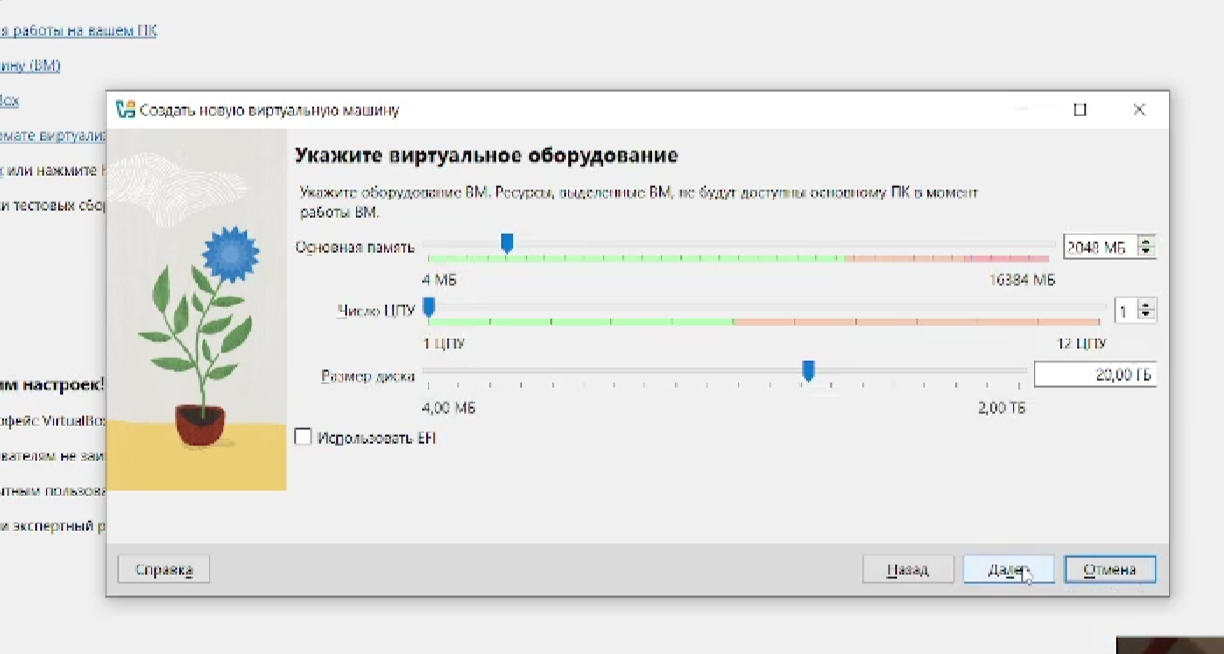
\includegraphics[width=0.7\textwidth,height=\textheight]{image/1.jpg}

}

\caption{\label{fig-001}Настройка ВМ}

\end{figure}%

Запускаю виртуальную машину , выбираю English в качестве языка
интерфейса и перехожу к настройкам установки операционной системы
(\textbf{?@fig-002}).

\begin{figure}

\centering{

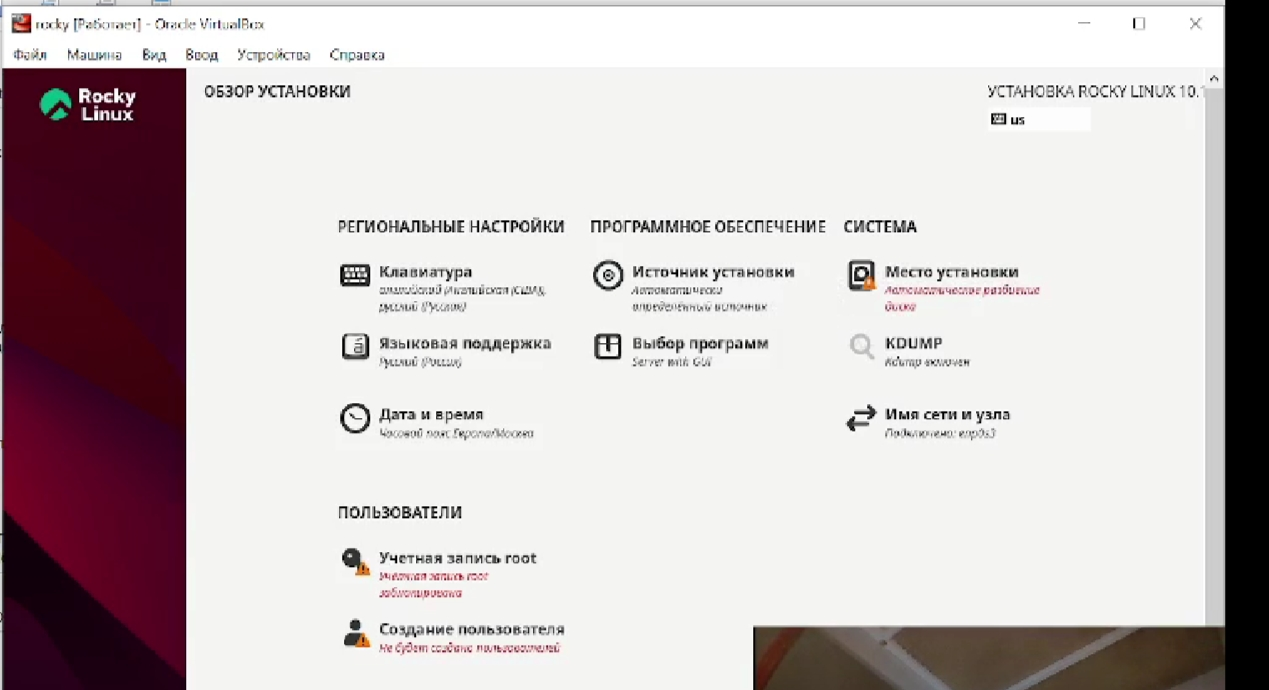
\includegraphics[width=0.7\textwidth,height=\textheight]{image/2.jpg}

}

\caption{\label{fig-003}Окно настройки установки образа ОС}

\end{figure}%

После завершения установки операционной системы корректно перезапускаю
виртуальную машину и при запросе принимаю условия лицензии
(рис.~\ref{fig-003}).

\begin{figure}

\centering{

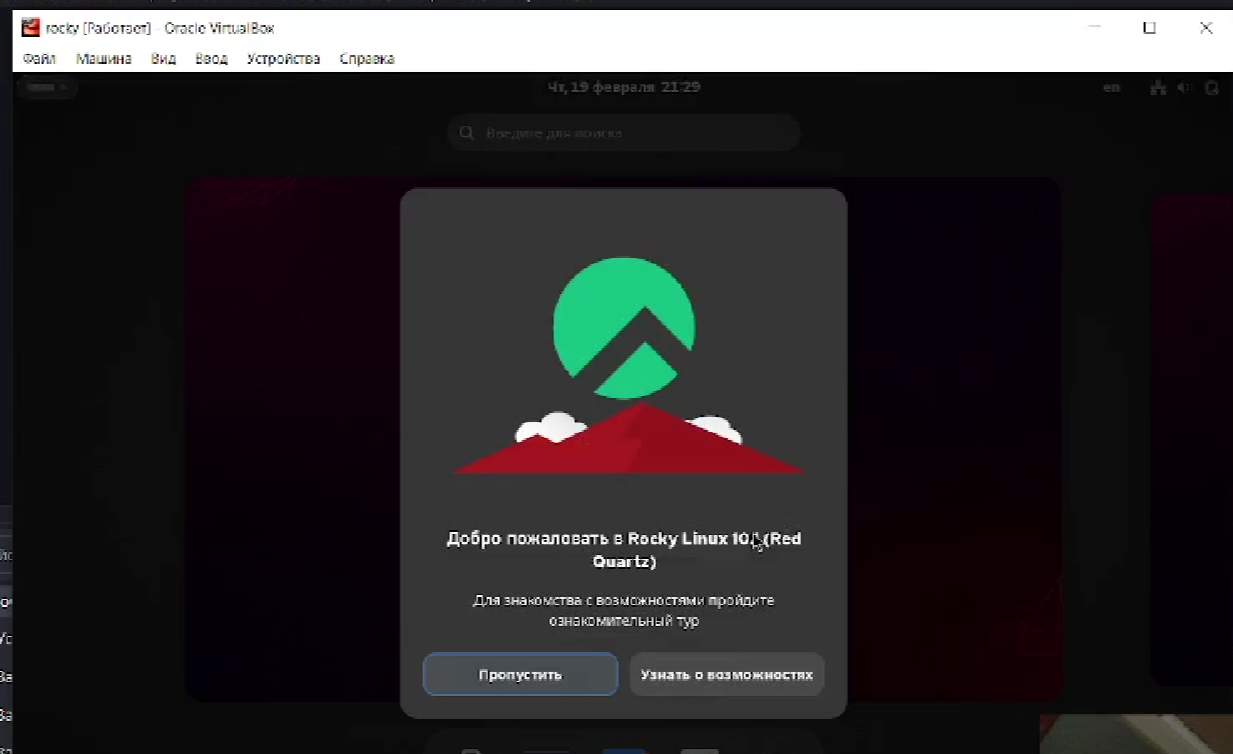
\includegraphics[width=0.7\textwidth,height=\textheight]{image/3.jpg}

}

\caption{\label{fig-003}Завершаю установку}

\end{figure}%

\#Вопросы

Версия ядра Linux: 6.12.0-124.8.1.el10\_1.x86\_64

Частота процессора: 2096.062 МГц

Модель процессора: AMD Ryzen 5 5500U with Radeon Graphics

Объем доступной оперативной памяти: 1200348 kB (примерно 1.14 ГБ)

Тип обнаруженного гипервизора: oracle (Oracle VM VirtualBox)

Тип файловой системы корневого раздела: xfs

\#Контрольные вопросы

\textbf{1. Какую информацию содержит учётная запись пользователя?} Имя
пользователя, UID, GID, домашний каталог, зашифрованный пароль,
командная оболочка, описание пользователя.

\textbf{2. Команды терминала и примеры:}

Справка по команде: man ls ls --help

Перемещение по файловой системе: cd /home cd .. cd \textasciitilde{} cd
-

Просмотр содержимого каталога: ls ls -l ls -a ls -lh

Определение объёма каталога: du -sh /home du -h df -h

Создание и удаление каталогов и файлов: mkdir newdir touch file.txt rm
file.txt rm -r newdir rmdir emptydir cp file.txt copy.txt mv file.txt
new.txt

Задание прав на файл или каталог: chmod 755 script.sh chmod u+x file.txt
chmod go-w file.txt chown user:group file.txt

Просмотр истории команд: history history 10 !! !100 Ctrl+R

\textbf{3. Что такое файловая система? Примеры с характеристикой.}
Файловая система определяет способ хранения и доступа к данным на диске.

ext4 --- журналируемая ФС, используется в Linux по умолчанию,
поддерживает большие файлы и тома. xfs --- высокопроизводительная
журналируемая ФС, хороша для больших файлов и высокой нагрузки. btrfs
--- современная ФС с поддержкой снапшотов, сжатия и проверки целостности
данных. ntfs --- ФС Windows, поддерживает большие файлы, журналирование,
права доступа. fat32 --- старая ФС, ограничение на размер файла 4 ГБ,
нет журналирования, совместима со всем.

\textbf{4. Как посмотреть, какие файловые системы подмонтированы в ОС?}
mount df -h findmnt cat /proc/mounts

\textbf{5. Как удалить зависший процесс?} Найти PID процесса: ps aux
\textbar{} grep имя\_процесса top pidof имя\_процесса

Отправить сигнал завершения: kill PID kill -9 PID pkill имя\_процесса
killall имя\_процесса

\chapter{Выводы}\label{ux432ux44bux432ux43eux434ux44b}

Я преобрела практические навыки установки операционной системы на
виртуальную машину, настройки минимально необходимых для дальнейшей
работы сервисов.

\chapter*{Список
литературы}\label{ux441ux43fux438ux441ux43eux43a-ux43bux438ux442ux435ux440ux430ux442ux443ux440ux44b}
\addcontentsline{toc}{chapter}{Список литературы}

\printbibliography[heading=none]





\end{document}
